\chapter{Theoretical study of algorithms}
\label{ch:fundamental}

In this study, we employ Visual Object Tracking (VOT) methods to address the problem of underwater object tracking. VOT plays a crucial role in tracking objects across video frames, allowing for continuous localization without prior category knowledge. This approach is essential for handling dynamic underwater environments, where objects may undergo significant appearance changes due to lighting variations, occlusions, and water turbulence.

The field of VOT encompasses a diverse range of algorithmic approaches, broadly categorized into traditional correlation filter-based methods and modern deep learning-based techniques. Correlation filter-based trackers leverage frequency-domain operations for efficient tracking [24; 25], whereas deep learning-based methods exploit the representational power of neural networks to enhance robustness against appearance variations and challenging environmental conditions [26; 27]. This section presents a comprehensive theoretical study of key tracking algorithms, providing insights into their underlying principles and methodologies.



\section{Minimum Output Sum of Squared Error (MOSSE)}
The Minimum Output Sum of Squared Error (MOSSE) tracker, introduced by Bolme et al. \cite{bolme2010visual}, represents a pioneering approach in correlation filter-based object tracking. MOSSE employs adaptive correlation filters to efficiently track objects in real-time while maintaining robustness against variations in illumination, occlusions, and background clutter.

\subsubsection{Formulation of MOSSE}
The fundamental objective of MOSSE is to learn an optimal correlation filter $w^*$ that minimizes the sum of squared errors between the actual output of the convolution operation and the desired response, typically modeled as a Gaussian function centered on the target location. The optimization problem is formulated as follows:

\begin{equation} \label{eq:mosse}
    \underset{w^*}{\arg\min} \sum_{i} \left\| f_i \odot w^* - y_i \right\|^2,
\end{equation}
where:
\begin{itemize}
    \item $f_i$ represents the extracted feature map from the $i$-th input frame,
    \item $w^*$ is the correlation filter to be learned,
    \item $y_i$ is the desired response map modeled by a Gaussian function,
    \item $\odot$ denotes element-wise multiplication.
\end{itemize}

\subsubsection{Solution in the Frequency Domain}
Direct computation in the spatial domain is computationally expensive. Leveraging the Convolution Theorem, which states that convolution in the spatial domain is equivalent to element-wise multiplication in the frequency domain, MOSSE reformulates the optimization problem using the Discrete Fourier Transform (DFT):

\begin{equation}
    \hat{w}_i = \frac{\sum_i \hat{y}_i \odot \hat{f}_i^*}{\sum_i \hat{f}_i \odot \hat{f}_i^*},
\end{equation}
where $\hat{\cdot}$ denotes the Fourier transform, and $(\cdot)^*$ represents the complex conjugate.

Once the optimal filter $\hat{w}_i$ is obtained, object localization in a new frame is determined by computing the response map:

\begin{equation}
    \hat{y}_m = \sum_{i=1}^{D} \hat{w}_i \odot \hat{f}_i.
\end{equation}

Applying the inverse Fourier transform recovers the response map in the spatial domain:

\begin{equation}
    y_m = \mathcal{F}^{-1}(\hat{y}_m).
\end{equation}

The target's new location is estimated as the coordinates of the maximum value in $y_m$ \cite{bolme2010visual}.

\subsubsection{Online Filter Update Mechanism}
To account for appearance variations such as lighting changes and partial occlusions, MOSSE employs an online filter update strategy. The filter numerator $A_i$ and denominator $B_i$ are updated adaptively using a learning rate $\eta$:

\begin{equation}
    \begin{aligned}
        A_i &= \eta \hat{y}_i \odot \hat{f}_i^* + (1 - \eta) A_{i-1}, \\
        B_i &= \eta \hat{f}_i \odot \hat{f}_i^* + (1 - \eta) B_{i-1}.
    \end{aligned}
\end{equation}

The updated filter for subsequent frames is computed as:
\begin{equation}
    \hat{w}_i = \frac{A_i}{B_i}.
\end{equation}

This adaptive mechanism enables MOSSE to maintain tracking performance despite dynamic changes in the target's appearance \cite{bolme2010visual}.

\subsubsection{Advantages and Limitations}
MOSSE is well-regarded for its computational efficiency, achieving high-speed tracking rates suitable for real-time applications. Key advantages include:
\begin{itemize}
    \item Robustness to lighting variations and partial occlusions,
    \item Efficient learning with a low computational footprint,
    \item Real-time performance with high frame rates.
\end{itemize}
However, MOSSE has limitations, particularly in handling:
\begin{itemize}
    \item Scale variations, as it assumes a fixed target size,
    \item Background clutter in complex tracking environments,
    \item Non-rigid object deformations.
\end{itemize}

\subsubsection{Conclusion}
MOSSE introduced a groundbreaking framework for object tracking using correlation filters, demonstrating real-time performance with adaptive learning. While its limitations have prompted the development of more advanced trackers, such as Kernelized Correlation Filters (KCF) \cite{henriques2014high}, MOSSE remains a foundational method in visual object tracking due to its simplicity and efficiency.



%%%%% KCF
%%%%%

\section{Kernelized Correlation Filter (KCF)}
The Kernelized Correlation Filter (KCF), introduced by Henriques et al. \cite{henriques2014high}, extends the MOSSE framework by incorporating the kernel trick to project image features into a higher-dimensional space. This non-linear transformation improves the discriminative power of the learned filter, enhancing tracking robustness against appearance variations such as scale changes, deformations, and occlusions \cite{henriques2012exploiting}.

Unlike MOSSE, which operates in the linear domain, KCF utilizes a kernel function $k(x, x')$ that implicitly maps the input data into a high-dimensional feature space without explicit computation. This allows for the use of more complex decision boundaries while maintaining computational efficiency through the use of circulant matrices and the Fast Fourier Transform (FFT) \cite{henriques2014high}.

The optimization problem in KCF follows a similar formulation to MOSSE but extends it using a kernel function:
\begin{equation}
    \underset{\alpha}{\arg\min} \sum_{i} \left\| \sum_{j} \alpha_j k(x_i, x_j) - y_i \right\|^2 + \lambda \|\alpha\|^2,
\end{equation}
where:
\begin{itemize}
    \item $k(x_i, x_j)$ is the kernel function measuring similarity between image patches $x_i$ and $x_j$.
    \item $\alpha$ represents the dual coefficients of the kernel function.
    \item $\lambda$ is a regularization parameter to prevent overfitting.
\end{itemize}

The solution to the above optimization problem in the Fourier domain is given by:
\begin{equation}
    \hat{\alpha} = \frac{\hat{y}}{\hat{k} + \lambda},
\end{equation}
where $\hat{k}$ is the Discrete Fourier Transform (DFT) of the kernelized correlation function \cite{henriques2014high}.

The most commonly used kernel in KCF is the Gaussian kernel:
\begin{equation}
    k(x_i, x_j) = \exp\left(-\frac{\|x_i - x_j\|^2}{2\sigma^2} \right),
\end{equation}
which ensures a smooth response map and improved tracking stability \cite{henriques2012exploiting}.

Once the optimal filter $\hat{\alpha}$ is learned, object localization in a new frame is determined via element-wise multiplication in the Fourier domain:
\begin{equation}
    \hat{y}_m = \hat{\alpha} \odot \hat{k}.
\end{equation}
Finally, the inverse Fourier transform is applied to recover the response map in the spatial domain:
\begin{equation}
    y_m = \mathcal{F}^{-1}(\hat{y}_m).
\end{equation}

The peak value of $y_m$ represents the object's estimated location in the current frame \cite{henriques2014high}.

\subsubsection{Scale Adaptation in KCF}
One limitation of the original KCF tracker is its inability to handle scale variations effectively. To address this, an improved version, known as KCF with scale estimation, introduces a multi-scale search mechanism \cite{danelljan2014accurate}. Instead of relying solely on fixed-size bounding boxes, KCF evaluates different scaled versions of the target appearance and selects the one with the highest response score.

The scale estimation process involves creating a set of scaled versions of the target patch and applying the learned correlation filter to each scale. The optimal scale $s^*$ is selected based on the peak response:
\begin{equation}
    s^* = \arg\max_s \mathcal{F}^{-1}(\hat{\alpha} \odot \hat{k}_s),
\end{equation}
where $\hat{k}_s$ represents the kernelized correlation response at scale $s$. This scale-adaptive mechanism significantly improves tracking performance in scenarios involving object size variations \cite{danelljan2016discriminative}.

\subsubsection{Enhancements in Feature Representations}
The original KCF tracker operates on raw intensity values, but subsequent implementations have incorporated more advanced feature representations, such as:
\begin{itemize}
    \item \textbf{Histogram of Oriented Gradients (HOG)}: Improves robustness to illumination and texture variations \cite{felzenszwalb2010object}.
    \item \textbf{Color Names (CN)}: Enhances performance in scenes with complex backgrounds \cite{danelljan2014adaptive}.
    \item \textbf{Deep Convolutional Features}: Extracted from pre-trained CNNs, allowing for superior target representation \cite{wang2015transferring}.
\end{itemize}
By integrating these features, modern KCF variants achieve significantly higher accuracy and robustness in real-world tracking applications.

\subsubsection{Computational Efficiency and Practical Considerations}
Despite its improvements, KCF remains computationally efficient due to its reliance on FFT and circulant matrix properties. The overall complexity remains $\mathcal{O}(n \log n)$, making it suitable for real-time applications \cite{henriques2014high}. However, practical considerations such as parameter tuning (e.g., regularization weight $\lambda$ and kernel bandwidth $\sigma$) can impact performance, requiring empirical optimization for different datasets \cite{danelljan2015learning}.

\subsubsection{Summary of KCF Improvements}
In summary, KCF extends MOSSE by introducing:
\begin{itemize}
    \item \textbf{Kernel methods} for improved discrimination \cite{henriques2014high}.
    \item \textbf{Scale adaptation} for handling object size variations \cite{danelljan2014accurate}.
    \item \textbf{Advanced feature representations} for better robustness \cite{wang2015transferring}.
    \item \textbf{Computational efficiency} suitable for real-time tracking \cite{henriques2014high}.
\end{itemize}
These enhancements make KCF a widely adopted approach in visual object tracking, balancing accuracy, robustness, and efficiency.



%%%%%%% GOTURN
%%%%%

\section{Generic Object Tracking Using Regression Networks (GOTURN)}
GOTURN, proposed by Held et al.\ \cite{held2016learning}, is a deep learning-based tracker that employs a regression network for fast and robust visual tracking. Unlike correlation filter-based approaches such as KCF, which rely on frequency domain operations, GOTURN formulates tracking as a bounding box regression problem, leveraging a deep convolutional neural network (CNN) to predict object motion from one frame to the next.

Unlike many conventional trackers that perform online adaptation, GOTURN is trained offline on a large dataset of labeled video sequences and images. This enables the tracker to generalize to novel objects at test time without requiring per-sequence fine-tuning \cite{held2016learning}. The model learns a generic mapping between object appearance and motion, making it significantly faster than traditional deep learning-based trackers that involve online learning \cite{held2016learning}.

\begin{figure}[h]
    \centering
    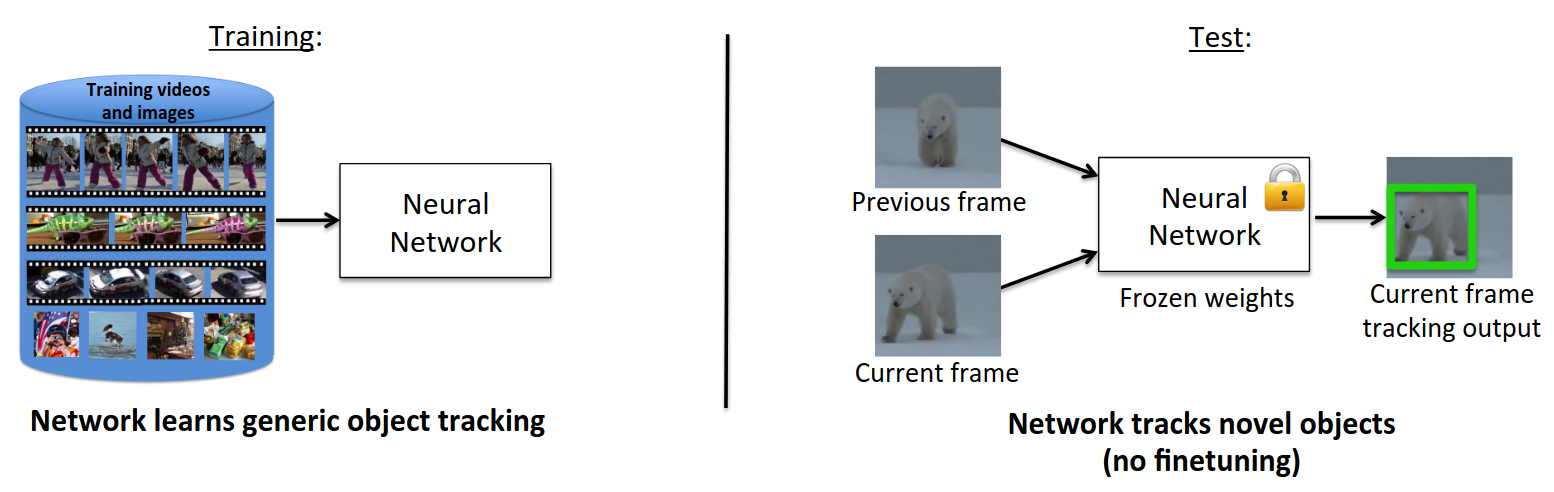
\includegraphics[width=1\linewidth]{images/GOTURN_OVERVIEW.png}
    \caption{A deep neural network is trained using a combination of labeled videos and images to track generic objects. At test time, the network generalizes to unseen objects without requiring fine-tuning, achieving real-time speeds of 100 FPS \cite{held2016learning}.}
    \label{fig:goturn_overview}
\end{figure}

\subsubsection{Network Architecture}
GOTURN consists of a CNN-based regression model that takes as input two consecutive image patches: the search region from the current frame and the target appearance from the previous frame. The network processes these inputs separately through a series of convolutional layers before merging them into a fully connected layer that outputs the coordinates of the tracked object's bounding box in the current frame \cite{held2016learning}.

\begin{figure}[h]
    \centering
    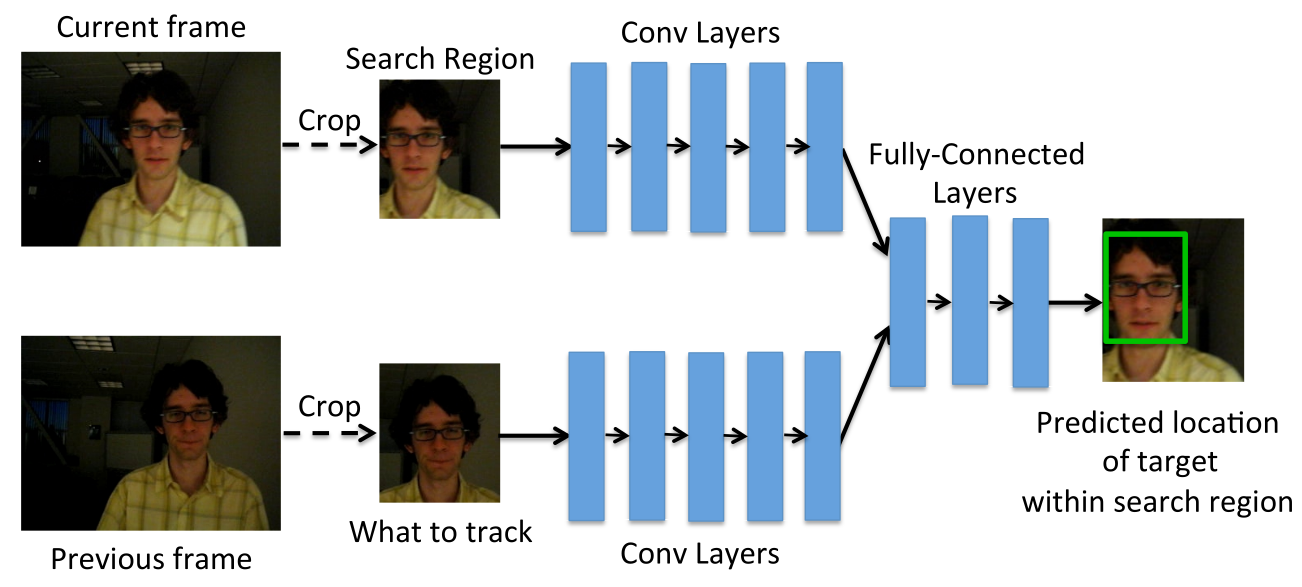
\includegraphics[width=1\linewidth]{images/goturn-architecture.png}
    \caption{The GOTURN architecture \cite{held2016learning}.}
    \label{fig:goturn_architecture}
\end{figure}

The architecture in Picture \ref{fig:goturn_architecture} follows a two-stream design:
\begin{itemize}
    \item The first stream extracts features from the target patch in the previous frame.
    \item The second stream extracts features from the search region in the current frame.
    \item The feature maps from both streams are concatenated and passed through fully connected layers to predict the new bounding box.
\end{itemize}

The convolutional layers are adapted from the CaffeNet architecture \cite{jia2014caffe}, which is a variant of AlexNet \cite{krizhevskyalexnet}. The final regression layer outputs the new bounding box coordinates relative to the search region \cite{held2016learning}.

\subsubsection{Loss Function and Training Strategy}
GOTURN uses an L1 loss function to minimize the difference between the predicted bounding box and the ground truth:
\begin{equation}
    L = \sum_{i=1}^{N} \left| \hat{b}_i - b_i \right|,
\end{equation}
where $b_i$ represents the ground-truth bounding box coordinates, and $\hat{b}_i$ denotes the predicted bounding box.

The network is trained on a combination of labeled video sequences and still images. The video sequences allow the model to learn temporal object motion, while the still images augment the training data by simulating motion via artificial transformations \cite{held2016learning}. The training data is further enhanced using a motion smoothness assumption, where small object movements are favored over large, abrupt changes, improving robustness to motion blur and occlusions.

\subsubsection{Tracking Mechanism}
During inference, GOTURN follows a simple tracking procedure:
\begin{enumerate}
    \item The tracker is initialized with a ground-truth bounding box in the first frame.
    \item For each subsequent frame, a search region centered around the previous bounding box is extracted.
    \item The network predicts the new bounding box coordinates within the search region.
    \item The predicted bounding box is used to update the target location.
\end{enumerate}
This approach allows GOTURN to operate without online fine-tuning, enabling real-time tracking at speeds up to 100 FPS on a GPU \cite{held2016learning}.

\subsubsection{Performance and Limitations}
GOTURN achieves state-of-the-art performance on the VOT-2014 benchmark \cite{held2016learning}, outperforming many traditional trackers in terms of accuracy and robustness. However, its reliance on offline training means it does not adapt to target appearance changes during tracking. Additionally, unlike correlation filter-based trackers such as KCF, it lacks an explicit scale estimation mechanism, making it less effective for tracking objects with large-scale variations \cite{danelljan2016discriminative}.

\subsubsection{Summary of GOTURN Contributions}
GOTURN introduces several key advancements in deep learning-based tracking:
\begin{itemize}
    \item \textbf{Offline training:} Unlike traditional trackers that learn online, GOTURN trains a deep network offline, improving speed and generalization \cite{held2016learning}.
    \item \textbf{Regression-based tracking:} Directly predicts bounding box locations using CNN-based feature extraction and fully connected regression layers \cite{held2016learning}.
    \item \textbf{Real-time performance:} Achieves up to 100 FPS, significantly faster than previous deep learning-based trackers \cite{held2016learning}.
\end{itemize}
Despite its limitations in handling appearance changes and scale variations, GOTURN remains a pioneering approach in deep learning-based object tracking, demonstrating the potential of regression networks for real-time applications.

\section{Siamese Region Proposal Network (SiamRPN)}
Siamese Region Proposal Network (SiamRPN), introduced by Li et al.\ \cite{li2018high}, is an extension of the Siamese network-based tracking framework that incorporates a region proposal network (RPN) for precise and efficient object localization. Unlike GOTURN, which directly regresses bounding box coordinates, SiamRPN applies a matching-based approach where the network learns a similarity function between the target template and candidate regions in the search space.

\subsubsection{Network Architecture}
SiamRPN follows a Siamese network design, consisting of two identical branches that extract deep feature embeddings from the target template and the search region. The key innovation in SiamRPN is the integration of an RPN module, which enables the network to generate multiple object proposals and select the most confident prediction \cite{li2018high}.

\begin{figure}[h]
    \centering
    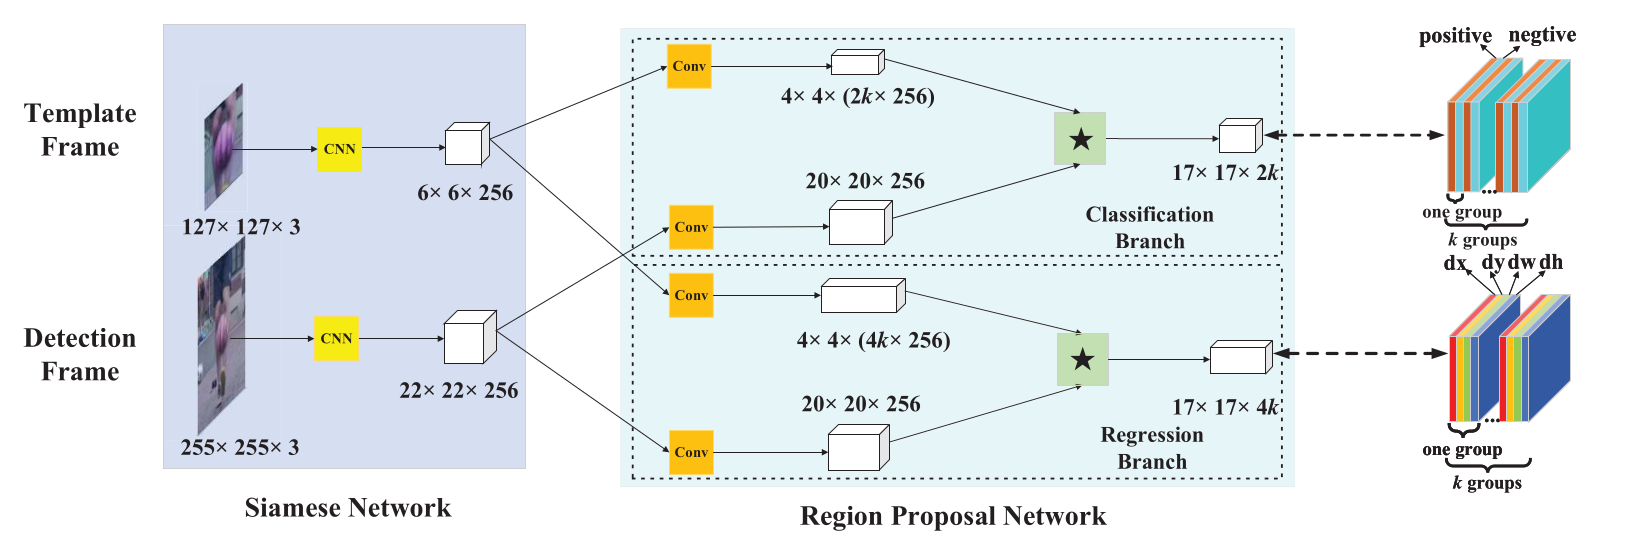
\includegraphics[width=1\linewidth]{images/SiamRPN-architechture.png}
    \caption{The SiamRPN architecture \cite{li2018high}.}
    \label{fig:siamrpn_architecture}
\end{figure}

The network operates as follows:
\begin{itemize}
\item The target template from the first frame is passed through a convolutional backbone (e.g., AlexNet or ResNet).
\item The search region from the current frame is processed through the same backbone.
\item A cross-correlation operation between the two feature maps is performed to compute response maps, representing object similarity.
\item The RPN module generates multiple anchor-based proposals and refines the bounding box predictions.
\end{itemize}
This pipeline enables SiamRPN to perform both localization and classification simultaneously, improving tracking accuracy compared to standard Siamese trackers such as SiamFC \cite{bertinetto2016fully}.

\subsubsection{Loss Function and Training Strategy}
SiamRPN optimizes a multi-task loss function, which includes:
\begin{equation}
L = L_{cls} + \lambda L_{reg},
\end{equation}
where:
\begin{itemize}
\item $L_{cls}$ is the classification loss, typically a cross-entropy loss for distinguishing target vs. background.
\item $L_{reg}$ is the bounding box regression loss, commonly a smooth L1 loss for refining object proposals.
\item $\lambda$ is a weighting factor to balance the two objectives.
\end{itemize}
Training SiamRPN requires large-scale video datasets with ground-truth annotations, such as ImageNet VID and YouTube-BB \cite{li2018high}. The network is pre-trained on static images and fine-tuned on video sequences to learn motion-aware representations.

\subsubsection{Performance and Advantages}
SiamRPN achieves state-of-the-art results on benchmarks such as OTB-2015 and VOT-2018, surpassing traditional trackers in terms of accuracy and robustness \cite{li2018high}. The main advantages of SiamRPN include:
\begin{itemize}
\item High-speed tracking: Runs at over 160 FPS due to efficient network design.
\item Robust localization: RPN improves bounding box estimation.
\item Scale adaptation: Handles object size variations better than fixed-scale trackers.
\end{itemize}
These characteristics make SiamRPN a widely used tracker in real-time applications, including autonomous driving and video surveillance.

\subsubsection{Comparison with GOTURN}
Compared to GOTURN, SiamRPN introduces several key improvements:
\begin{itemize}
\item Matching-based tracking (SiamRPN) vs. regression-based tracking (GOTURN).
\item Anchor-based bounding box proposals vs. direct bounding box prediction.
\item Better scale handling due to multi-scale region proposals.
\end{itemize}
Overall, SiamRPN represents a significant advancement in deep learning-based tracking, combining the efficiency of Siamese networks with the precision of RPN-based object detection.

\subsubsection{Variants of SiamRPN}

Following the success of SiamRPN, several improvements have been proposed to enhance its tracking performance, robustness, and efficiency. These variants introduce modifications to the backbone, region proposal strategy, and feature aggregation techniques.

\textbf{SiamRPN++} \cite{li2019siamrpn++} improves upon SiamRPN by utilizing deeper backbones such as ResNet and introducing spatial-aware sampling strategies to mitigate the limitations of small receptive fields in shallow networks. The network also applies depth-wise separable convolutions to enhance efficiency, making it more robust to large-scale variations.

\textbf{SiamBAN (Balanced Anchor-free Network)} \cite{chen2020siamban} replaces the anchor-based RPN module with an anchor-free mechanism, reducing computational complexity while improving accuracy. Instead of predefined anchor boxes, SiamBAN directly predicts the target’s center location and bounding box size, enhancing adaptability to scale variations.

\textbf{SiamCAR (Classification and Regression)} \cite{guo2020siamcar} further refines the anchor-free tracking paradigm by employing a dense prediction strategy. The network jointly classifies and regresses bounding boxes at each location in the feature map, improving tracking precision while maintaining high speed.

\textbf{LightTrack} \cite{yan2021lighttrack} emphasizes lightweight and efficient tracking by employing neural architecture search (NAS) to design a compact and optimized network. By balancing accuracy and computational efficiency, LightTrack achieves competitive performance while being well-suited for deployment on resource-constrained devices such as mobile and edge platforms.

\textbf{SiamGAT} \cite{lu2023siamese} introduces graph attention networks (GATs) into the Siamese tracking framework, allowing the model to better capture spatial relationships between objects and background features. This enhances tracking performance in cluttered scenes and improves robustness to occlusion.

\section{Transformer Tracker}
Transformer-based models have recently emerged as powerful alternatives to conventional correlation-based tracking frameworks. Unlike traditional approaches such as MOSSE \cite{bolme2010visual} and KCF \cite{henriques2014high}, which rely on handcrafted features and linear correlation, or deep-learning-based methods like SiamRPN \cite{li2018high} and GOTURN \cite{held2016learning}, which incorporate convolutional networks for feature extraction, Transformer-based tracking frameworks leverage self-attention mechanisms to enhance feature fusion and robustness.


\begin{figure}[h]
    \centering
    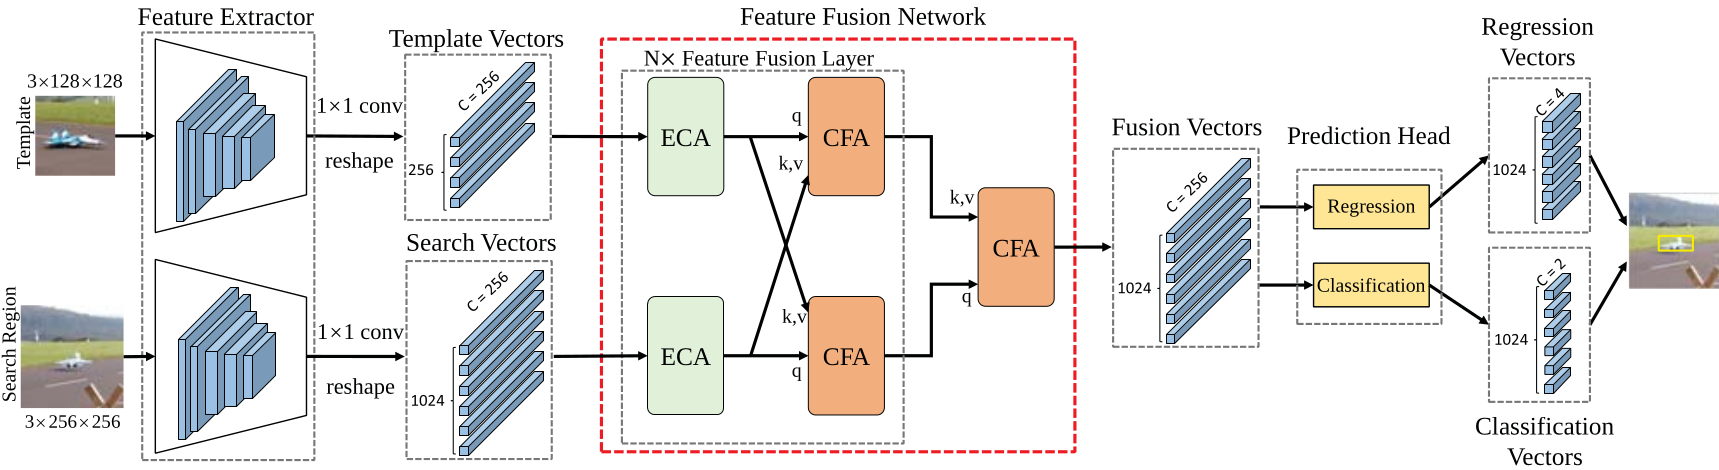
\includegraphics[width=1\linewidth]{images/vitt_architecture.png}
    \caption{Architecture of Transformer tracking framework \cite{chen2021transformer}.}
    \label{fig:transt_architecture}
\end{figure}

\subsubsection{Network Architecture} 
The Transformer architecture, originally proposed for natural language processing \cite{vaswani2017attention}, has been successfully adapted for object tracking. The core idea behind Transformer tracking is the replacement of the conventional cross-correlation operation with an attention-based feature fusion mechanism. One notable example is TransT \cite{chen2021transformer}, which introduces an attention-driven network consisting of an ego-context augment module (ECA) and a cross-feature augment module (CFA). These components effectively enhance global feature interactions between the target template and the search region.


\textbf{Feature Extraction:} Transformer-based trackers typically utilize a Siamese backbone for feature extraction. Given an input template $z \in \mathbb{R}^{3 \times H_z \times W_z}$ and a search region $x \in \mathbb{R}^{3 \times H_x \times W_x}$, a shared feature extractor (often based on ResNet-50 \cite{he2016deep}) processes both inputs to generate feature maps $f_z$ and $f_x$, which are then forwarded to the feature fusion network.

\textbf{Attention-Based Feature Fusion: }Unlike previous methods that apply depthwise cross-correlation for similarity computation, Transformer trackers employ self-attention and cross-attention modules:
\begin{itemize}
    \item \textbf{Ego-Context Augment (ECA):} Enhances local features by capturing long-range dependencies within the template and search region through multi-head self-attention.
    \item \textbf{Cross-Feature Augment (CFA):} Establishes interdependencies between template and search region features, allowing adaptive fusion without explicit correlation operations.
\end{itemize}

% ECA and CFA modules
\begin{figure}[h]
    \centering
    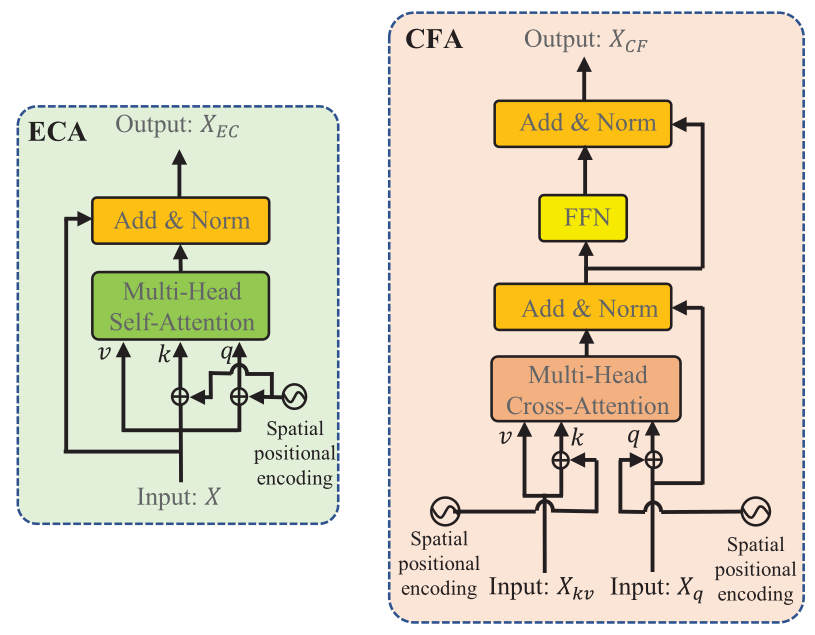
\includegraphics[width=0.8\linewidth]{images/ecs-cfa.png}
    \caption{Ego-Context Augment (ECA) and Cross-Feature Augment (CFA) modules in Transformer tracking \cite{chen2021transformer}.}
    \label{fig:eca_cfa}
\end{figure}

These attention modules enable the tracker to dynamically focus on salient regions of the target, mitigating issues like distractors and occlusion.

\textbf{Prediction Head: }The final stage of the Transformer tracker consists of a classification and regression network that predicts the target's presence and bounding box coordinates. Compared to conventional anchor-based regression techniques used in SiamRPN \cite{li2018high}, Transformer trackers such as TransT \cite{chen2021transformer} adopt a more flexible and parameter-free prediction mechanism, improving robustness against scale variations.

\subsubsection{Loss Function and Training Strategy}
The loss function for Transformer-based tracking is typically a combination of classification and regression losses:
\begin{equation}
L = L_{\text{cls}} + \lambda_{1} L_{\text{IoU}} + \lambda_{2} L_{1}
\end{equation}
where $L_{\text{cls}}$ is the binary cross-entropy loss for classification, $L_{\text{IoU}}$ is the IoU loss for bounding box regression, and $L_{1}$ is the smooth $l_1$ loss. Training is performed using datasets such as LaSOT, GOT-10k, and TrackingNet, with an AdamW optimizer and learning rate scheduling strategies.

\subsubsection{Performance and Advantages}
Transformer-based tracking approaches have demonstrated superior performance on large-scale benchmarks such as LaSOT, TrackingNet, and GOT-10k. Experimental results from \cite{chen2021transformer} indicate that TransT outperforms prior state-of-the-art trackers in terms of Average Overlap (AO) and Success Rate (SR) while maintaining real-time processing speeds (approximately 50 FPS on GPU).

\subsubsection{Comparison with CNN-Based Tracker}
Unlike CNN-based trackers, which rely heavily on handcrafted correlation operations, Transformer trackers leverage self-attention mechanisms that adaptively aggregate features across long spatial distances. This enables improved target localization, especially in scenarios involving occlusion, motion blur, and background clutter. Transformer-based methods also eliminate the need for predefined anchor boxes, leading to a more flexible and efficient tracking pipeline.

\subsubsection{Conclusion}
Transformer-based tracking represents a significant leap forward in visual object tracking, replacing handcrafted correlation operations with adaptive attention mechanisms. The ability to model long-range dependencies and adaptively fuse features makes these models particularly effective in challenging scenarios. Future work may explore hybrid architectures that integrate Transformer attention with convolutional inductive biases to further enhance tracking efficiency and robustness.




\endinput